\chapter{Warstwa pośrednia w zastosowaniu }
\label{cha:example}

Najlepszym sposobem weryfikacji każdego rozwiązania jest jego konfrontacja z rzeczywistością, przez znalezienie realnych przykładów jego użycia. Nie inaczej jest w przypadku proponowanego w niniejszej pracy rozwiązania. 

Pomysłem na przykład jest w tym przypadku proces sprzątania pokoju hotelowego. Celem przykładu jest zademonstrowanie działania warstwy pośredniej do komunikacji procesu biznesowego z aplikacjami mobilnymi, ale również pokazania sposobu integracji takiego rozwiązania z gotowymi systemami zewnętrznymi. 

%---------------------------------------------------------------------------

\section{Przedstawienie koncepcji}
\label{sec:concept}

Prezentacja przykładu zostanie rozpoczęta od przedstawienia koncepcji rozwiązania w postaci diagramów zaprojektowany za pomocą BPMN 2.0. Przedstawione zostaną dwa diagramy z których pierwszy jest sytuacją w której rozpoczyna się właściwy proces sprzątania hotelu. 

\begin{figure}[h]
\centerline{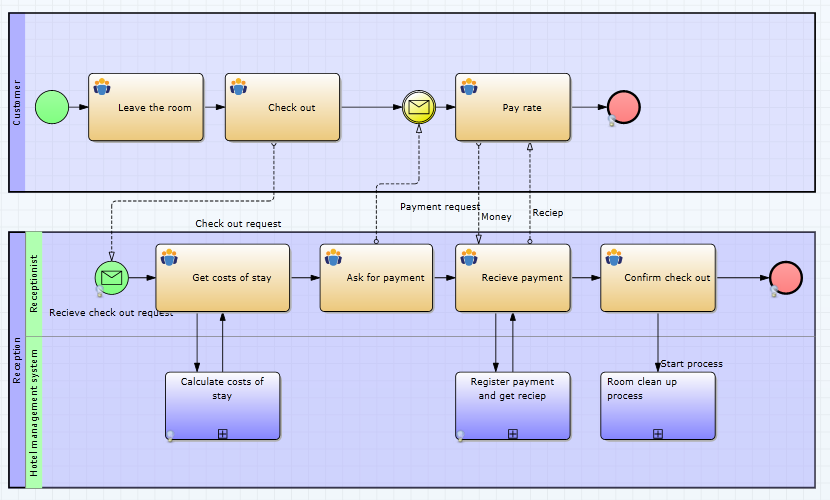
\includegraphics[scale=0.4]{hotelCheckOutProcess}}
\caption{Diagram BPMN procesu wymeldowania klienta z pokoju hotelowego.}
\label{fig:hotelCheckOutProcess}
\end{figure}

Na rysunku ~\ref{fig:hotelCheckOutProcess}, przedstawiono proces wymeldowania gościa hotelowego z pokoju po zakończonym pobycie. Klient hotelu po opuszczeniu pokoju udaje się do recepcji w celu oddania kluczy i uregulowania płatności. W recepcji przebywa recepcjonista, który odpowiedzialny jest za kontakt z klientem, o otrzymaniu kluczy prosi klienta o zapłatę kosztów pobytu. Po wymianie płatności na rachunek klient hotelowy opuszcza hotel, a recepcjonista oznacza pokój hotelowy jako gotowy do posprzątania, rozpoczynając w ten sposób właściwy proces. 

\begin{figure}[h]
\centerline{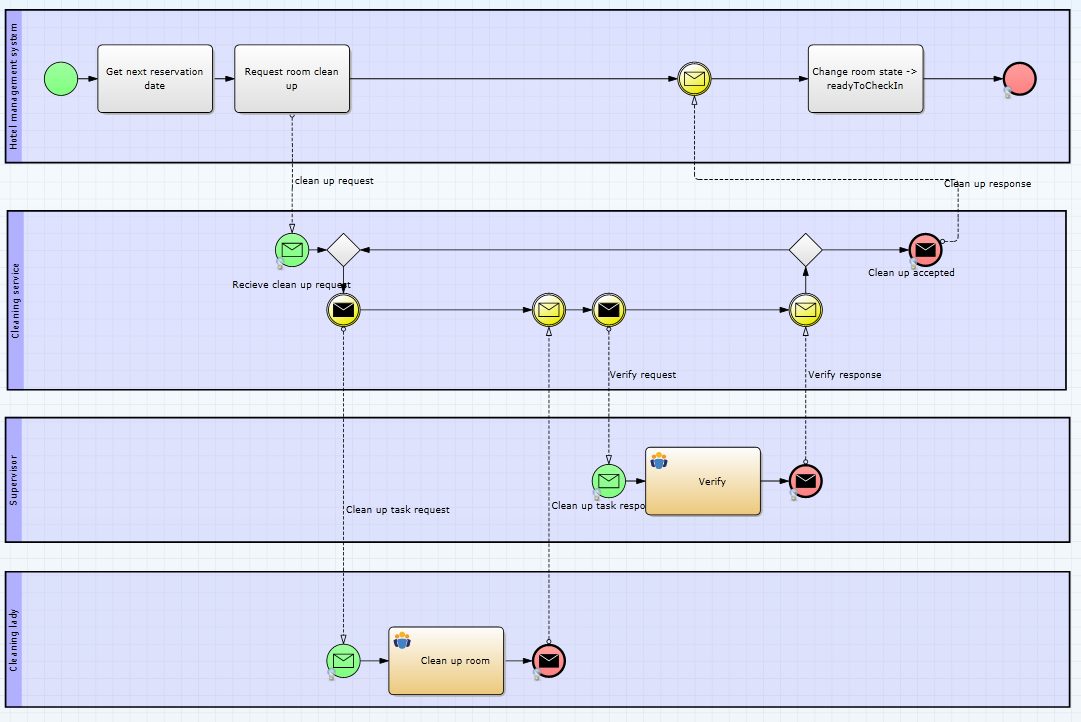
\includegraphics[scale=0.4]{roomCleanUpProcess}}
\caption{Diagram BPMN procesu sprzątania pokoju hotelowego.}
\label{fig:roomCleanUpProcess}
\end{figure}

Rysunek~\ref{fig:roomCleanUpProcess} przedstawia właściwy proces sprzątania pokoju hotelowego, widzimy na nim cztery rodzaje aktorów, każdy z nich oznaczony własną linią. Pierwszym z aktorów jest system zarządzania hotelem, jest to miejsce w którym recepcjonista oznacza pokój do posprzątania. System zarządzania hotelem jest miejscem w którym rozpoczyna się proces. Odpowiedzialny jest on za zebranie danych koniecznych do przeprowadzenia sprzątania a następnie przekazanie tych danych do kolejnego aktora, którym jest Serwis Sprzątający. A przypadku realizacji przykładu za pomocą opisanych w niniejszej pracy magisterskiej technologii aktora tego można utożsamić z procesem BPEL wraz z warstwą pośrednią. Serwis sprzątający odpowiedzialny jest za przeprowadzenie procesu sprzątania. Proces ten odbywa się przez wysłanie żądania do sprzątaczki (aplikacja mobilna), by po potwierdzeniu posprzątania pokoju wysłać żądanie do nadzorcy (również aplikacja mobilna) który będzie odpowiedzialny za weryfikacje sprzątania.  W przypadku braku akceptacji sprzątania przez nadzorcę pokój będzie musiał być kolejny raz posprzątany. W momencie zatwierdzenia sprzątania, rezultat trafi ponownie do Systemu Zarządzania Hotelem, aby recepcjonista mógł zameldować kolejnych gości. 

Na podstawie opisanego powyżej przykładu wyłonić można następujące systemy, których implementacja zostanie dokładniej opisana w dalszej części pracy.

\begin{itemize}
\item System Zarządzania Hotelem -- Dla celów przykładu, System Zarządzania Hotelem będzie prosta aplikacją internetową odpowiedzialną za udostępnienie formularza dla recepcjonisty oraz wyświetlenie listy rezultatów wykonania procesu.   
\item Proces BPEL -- Będzie to proces zawierający kompletną logikę biznesową odpowiedzialną za przeprowadzenie i weryfikacje sprzątania pokoju hotelowego. Proces ten będzie komunikował się zarówno z warstwą pośrednią jak i z Systemem Zarządzania Hotelem. 
\item Warstwa pośrednia --  Aplikacja internetowa odpowiedzialna za obsługę komunikacji procesu biznesowego z aplikacjami mobilnymi. 
\item Aplikacja mobilna -- aplikacja przeznaczona zarówno dla sprzątaczek jak i dla nadzorców. Udostępniać będzie bardzo prosty interfejs użytkownika służący do wyświetlenia listy zadań oraz do ich przypisywania i rozwiązywania. 
\end{itemize}


%---------------------------------------------------------------------------

\section{System Zarządzania Hotelem }
\label{sec:hotelManagementSystem}

Zadaniem tej aplikacji jest udostępnienie części funkcjonalność Systemu Zarządzania Hotelem przeznaczonej do oznaczania pokoju hotelowego jako wymagającego posprzątania. Aplikacja udostępniać będzie formularz w którym recepcjonista będzie mógł zgłosić pokój do posprzątania. Formularz będzie gromadził taki dane jak numer pokoju, numer piętra oraz kategorię do której należy pokój. Po zatwierdzeniu formularza  dane z niego pochodzące trafią do procesu biznesowego oraz do bazy danych w celu monitorowania postępu procesu. Kiedy proces zakończy swoje działania aplikacja odbierze za pomocą odpowiedniej usługi sieciowej jego rezultat. Odebranie rezultatu skutkować będzie zmianą statusu pokoju. Aplikacja udostępniać będzie również listę pokoi wraz z ich statusami w postaci strony html. 

\subsection{Wybrane technologie}
Aplikacja zostanie zrealizowana przy wykorzystaniu technologii:

\begin{itemize}
\item język programowania Java
\item Spring MVC
\item  Bootstrap Framework -- jest to zbiór  klas css oraz biblioteka stworzona w języku JavaScript, służący do tworzenia interfejsu użytkownika przy pomocy zaawansowanych kontrolek html.
\item Maven
\item Spring Web Services
\item Spring Data oraz Hibernate - jeden z najbardziej popularnych narzędzi ORM, przeznaczonych na platformę Java. 
\item H2 in memory - baza danych której cykl życia jest równoznaczny z cyklem życia aplikacji. Jest ona tworzona podczas uruchamiana aplikacji, dane znajdujące w się w niej są przechowywane w pamięci podręcznej. Bazy tego typu wykorzystywane są przede wszystkim do implementacji testów jednostkowych. Zdecydowanym plusem skorzystania z tego rodzaju bazy danych jest brak konieczności instalacji dodatkowych narzędzi co w przypadku niniejszego przykładu jest dużym udogodnieniem. 
\end{itemize}

\subsection{Implementacja}

\begin{figure}[h]
\centerline{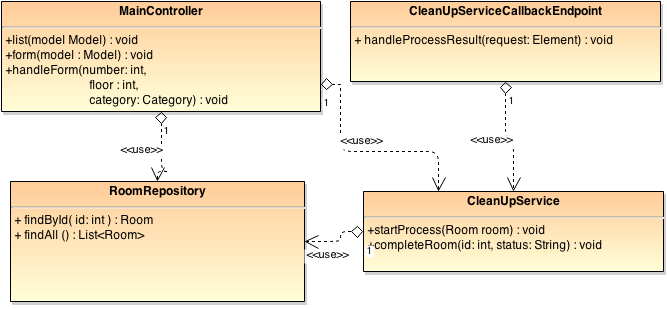
\includegraphics[scale=0.6]{hotelManagementSystemClasses}}
\caption{Diagram klas systemu zarządzania hotelem.}
\label{fig:hotelManagementSystemClasses}
\end{figure}


Na rysunku~\ref{fig:hotelManagementSystemClasses} został przedstawiony diagram klas Systemu Zarządzania Hotelem. Znajdują się na nim jedynie najbardziej istotne klasy z punku widzenia tej implementacji. Klasa MainController jest odpowiedzialna za udostępnienie interfejsu użytkownika oraz za obsługę żądań z niego pochodzących. Udostępnia ona trzy metody: 


\begin{itemize}
\item list -- metoda za pomocą RomRepository pobiera z bazy danych wszystkie pokoje, które zostały zgłoszone do posprzątania. Pobrana lista jest  następnie umieszczana w dynamicznej stronie html za pomocą technologii JSP. 
\item form -- metoda odpowiedzialna za wyświetlenie formularza w postaci html dla użytkownika. 
\item hadleForm -- metoda ta jest uruchamiana w przypadku zatwierdzenia danych wprowadzonych do formularza przez użytkownika. Metoda dodaje nowy pokój do bazy danych oraz uruchamia proces biznesowy z wykorzystaniem klasy CleanUpService. 
\end{itemize}

Druga bardzo ważną klasą jest CleanUpServiceCallbackEndpoint, jest to klasa stworzona z wykorzystaniem technologii Spring Web Services. Klasa ta obsługuje zdefiniowaną w konfiguracji usługę sieciową. Usługa służy do odbierania rezultatów wykonania procesu biznesowego. Jej rolą jest przeczytania komunikatu przysłanego przez proces biznesowy by następnie zmienić status sprzątanego pokoju za pomocą klasy CleanUpService. 

\subsection{Uruchomienie}

Aplikacja jest kompilowana do postaci pliku o rozszerzeniu war. Pliki tego typu mogą być uruchamiana na dowolnym serwerze aplikacyjnym Java, np. Tomcat. Aplikacja powinna zostać uruchomiona na porcie 8181, ponieważ pozostałe aplikacje będą od niej tego wymagały. Np. proces biznesowy swój rezultat będzie wysyłał właśnie do lokalnej maszyny właśnie na ten port. 

%---------------------------------------------------------------------------

\section{Proces BPEL }
\label{sec:exampleBPEL}

Proces BPEL jest odpowiedzialny za obsługę logiki biznesowej związanej z przeprowadzeniem procesu sprzątania. Proces służy w pewnym sensie jako narzędzie integracyjne aplikację internetową jaką jest System Zarządzania Hotelem z aplikacjami mobilnymi. 

Przebieg działania procesu rozpoczyna się w Systemie Zarządzania Hotelem, który uruchamia usługę sieciową udostępnianą jako punkt dostępowy procesu. Proces po otrzymaniu żądania z systemu zewnętrznego tworzy nowe zadanie przeznaczone dla osoby sprzątającej pokój by następnie przejść w tryb oczekiwania na jego rezultat. Gdy pokój zostanie posprzątany, proces tworzy kolejne zadanie tym razem przeznaczone dla nadzorcy i ponownie przechodzi w tryb oczekiwania na jego rezultat. Gdy nadzorca zakończy swoje zadanie proces sprawdzi jego rezultat, jeśli sprzątanie pokoju zostało zaakceptowane proces zakończy swoje działanie poprzez wysłanie rezultatu do Systemu Zarządzania Hotelem. Gdy sprzątanie pokoju nie zostanie zaakceptowane proces będzie tworzył  kolejne zadania dla osoby sprzątającej do momentu zatwierdzenia przez nadzorcę. 


\subsection{Implementacja}

\begin{figure}[h]
\centerline{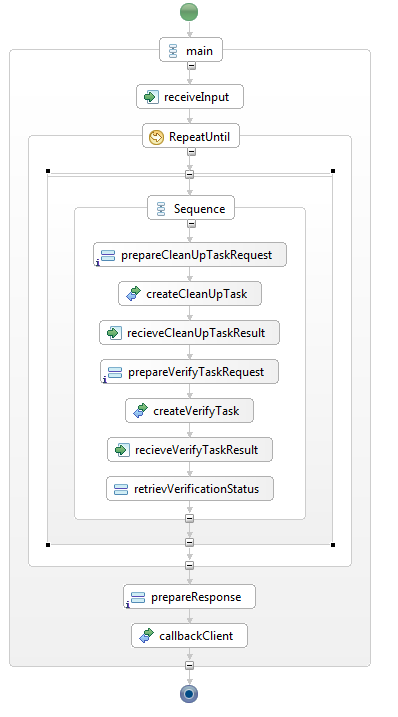
\includegraphics[scale=0.6]{bpelProcess}}
\caption{Wizualizacja procesu BPEL w postaci graficznej za pomocą wtyczki do Eclipsa.}
\label{fig:bpelProcess}
\end{figure}

Do implementacji procesu BPEL została wykorzystana wtyczka do zintegrowanego środowiska programistycznego Eclipse. Wtyczka ta udostępnia narzędzia do modelowania procesów BPEL w sposób graficzny. Na rysunku~\ref{fig:bpelProcess} został przedstawiony zrzut ekranu przedstawiający implementację niniejszego procesu biznesowego. Na rysunku widać doskonale kolejność wywoływania poszczególnych aktywności procesu BPEL, nie widać natomiast zastosowania mechanizmu korelacji oraz zakresu. 

\subsubsection{Korelacja}

Mechanizmem na który w szczególności należy zwrócić uwagę podczas opisu procesu biznesowego jest mechanizm korelacji. Mechanizm ten służy do powiązania dwóch lub więcej operacji wewnątrz jednej instancji procesu. W przypadku niniejszego przykładu proces korelacji wykorzystywany jest do powiązywania operacji stworzenie zadania z operacją odebrania rezultatu zadania. Zazwyczaj środowisko uruchomieniowe posiada więcej niż jedną instancje procesu, w momencie gdy zostaje odebrany rezultat zadania np. sprzątania środowisko powinno w jakiś sposób zidentyfikować instancję procesu do której zaadresowany jest ten rezultat. 

Mechanizm korelacji realizowany jest za pomocą tak zwanych zbiorów korelacji. Zbiór korelacji nie jest niczym innym jak zbiorem zmiennych. Zmienne te inicjalizowane są przy pierwszym użyciu dowolną wartością, podczas kolejnego użycia służą do odszukania instancji procesu o zadanej wartości. 

W niniejszym procesie istnieją dwa zbiory korelacji, zdefiniowane wewnątrz ciała pętli: 

\begin{lstlisting}[caption=Definicja zbiorów korelacji.,numbers=left]
<bpel:correlationSets>
	<bpel:correlationSet name="cleanUpTask" 
			properties="tns:taskUUID"/>
	<bpel:correlationSet name="verifyTask" 
			properties="tns:verifyTaskUUID"/>
</bpel:correlationSets> 


\end{lstlisting}

Zbiory te wykorzystywane są do powiązania operacji stworzenia i odbioru rezultatu zadania sprzątanie i weryfikacja. 

\begin{lstlisting}[caption=Wykorzystanie zbiorów korelacji w aktywności invoke.,numbers=left]
<bpel:receive name="recieveCleanUpTaskResult" partnerLink="client" 
	operation="cleanUpTaskCallback" portType="tns:cleanUpProcess" 
	variable="clientRequest">
            <bpel:correlations>
                <bpel:correlation set="cleanUpTask" initiate="no">
	     </bpel:correlation>    
            </bpel:correlations>
        
</bpel:receive>
\end{lstlisting}

Operacja invoke odpowiedzialna za stworzenie zadania inicjalizuje zbiór korelacji odebraną z warstwy pośredniej wartością unikalnego identyfikatora zadania.

\begin{lstlisting}[caption=Wykorzystanie zbiorów korelacji w aktywności receive.,numbers=left]
<bpel:receive name="recieveCleanUpTaskResult" partnerLink="client" 
		operation="cleanUpTaskCallback"
	          portType="tns:cleanUpProcess" variable="clientRequest">
            <bpel:correlations>
                	<bpel:correlation set="cleanUpTask" initiate="no">
		</bpel:correlation>    
            </bpel:correlations>
</bpel:receive>

\end{lstlisting}

 Operacja recieve następnie na podstawie tego samego unikalnego identyfikatora odnajduje odpowiednią instancje by kontynuować jej działanie. 

\subsubsection{Zakres }
Bezpośrednio powiązany z mechanizmem korelacji jest mechanizm zakresów. Służy on do odizolowania dwóch lub więcej operacji wewnątrz procesu. Izolacja ta może zostać wykorzystana np. do odpowiedniego zarządzania sytuacjami wyjątkowymi. W przypadku niniejszego procesu mechanizm zakresu został zastosowany do odizolowania kolejnych wywołań pętli w celu uzyskania efektu ponownej inicjalizacji zbiorów korelacji w każdym przebiegu pętli. W przypadku nie zastosowania mechanizmy zakresu, podczas pierwszego wywołania przebiegu pętli zbiór korelacji zostałby zainicjalizowany identyfikatorem pierwszego zadania. W przypadku kolejnych wywołań pętli metoda reciev oczekiwała by na identyfikator pierwszego zadania mimo, że zostało ono już rozwiązane a kolejny przebieg pętli stworzył następne zadanie. 

Mechanizm zakresu stosuje się obejmując izolowane elementy w drzewie xml elementem: 

\begin{lstlisting}[caption=Przykład zastosowania zakresu w BPEL.,numbers=left]
<bpel:scope isolated="yes">
...
</bpel:scope>
\end{lstlisting}

\subsection{Uruchomienie}
 Proces BPEL został stworzony zgodnie ze specyfikacją BPEL, może być zatem wdrożony na dowolne środowisko uruchomieniowe dla procesów biznesowych. W przykładzie zastosowano środowisko Apache ODE. 

Apache ODE jest również aplikacją internetową napisaną w języku Java i może być uruchomiony z wykorzystaniem dowolnego serwera aplikacyjnego. Ważne jest aby silnik Apache ODE został uruchomiony z wykorzystaniem portu 8080. System Zarządzania Hotelem będzie próbował uruchomić proces na lokalnej maszynie pod tym właśnie portem.  


%---------------------------------------------------------------------------

\section{Warstwa pośrednia }
\label{sec:exampleMiddleware}


%---------------------------------------------------------------------------

\section{Aplikacja mobilna}
\label{sec:exampleMobileApp}

Aplikacja mobilna jest częścią przykładu odpowiedzialną za rozwiązywanie zadań poprzez udostępnienie użytkownikom odpowiedniego interfejsu. Aplikacja komunikuje się w warstwą pośrednią za pomocą REST API w celu pobrania listy zadań, operacji na tych zadaniach i wysłania rezultatu. Aplikacja została zaimplementowana na najbardziej popularną platformę mobilną - Android. 

Aplikacja wykorzystuje specyficzny dla tej platformy mechanizm synchronizacji zarządzany przez system operacyjny. Synchronizacja uruchamiana jest bez konieczności działania aplikacji w momencie gdy urządzenie ma dostęp do sieci. Przez synchronizacje w tym wypadku rozumiane jest pobranie listy zadań dostępnych dla użytkownika i ich zapis w lokalnej bazie danych (SQLite). Aplikacja przewiduje możliwość logowania więcej jak jednego użytkownika, dane każdego z nich zapisywane są do osobnej bazy danych. Użytkownik po wejściu do aplikacji widzi listę dostępnych dla niego zadań mimo, że może nie mieć dostępu do sieci. Użytkownik może zadeklarować chęć wykonania zadania oraz w momencie gdy jest do niego przypisany rozwiązać je klikając odpowiednie przyciski.

\subsection{Wybrane technologie}

Aplikacja została zrealizowana z wykorzystaniem język Java, platformy Android, bibliotek Spring  for Android oraz OrmLite. 

\subsection{Implementacja}